\documentclass[a4paper,ngerman,12pt]{scrreprt}

% Packages required by doxygen
\usepackage{fixltx2e}
\usepackage{calc}
\usepackage{doxygen}
\usepackage[export]{adjustbox} % also loads graphicx
\usepackage{graphicx}
\usepackage[utf8]{inputenc}
\usepackage{makeidx}
\usepackage{multicol}
\usepackage{multirow}
\usepackage{textcomp}
\usepackage[nointegrals]{wasysym}
\usepackage[table]{xcolor}
% NLS support packages
\usepackage[ngerman]{babel}
\usepackage{tabularx}
% Font selection
\usepackage[T1]{fontenc}
\usepackage[scaled=.90]{helvet}
\usepackage{courier}
\usepackage{amssymb}
\usepackage{sectsty}
\usepackage[printonlyused,withpage,footnote]{acronym}
\usepackage[shortlabels]{enumitem}

\renewcommand{\familydefault}{\sfdefault}
\allsectionsfont{%
	\fontseries{bc}\selectfont%
	\color{darkgray}%
}
\renewcommand{\DoxyLabelFont}{%
	\fontseries{bc}\selectfont%
	\color{darkgray}%
}
\newcommand{\+}{\discretionary{\mbox{\scriptsize$\hookleftarrow$}}{}{}}

% Page & text layout
\usepackage{geometry}
\geometry{%
	a4paper,%
	top=2.5cm,%
	bottom=2.5cm,%
	left=2.5cm,%
	right=2.5cm%
}
\tolerance=750
\hfuzz=15pt
\hbadness=750
\setlength{\parindent}{0cm}
\setlength{\parskip}{3ex plus 2ex minus 2ex}
\makeatletter
\renewcommand{\paragraph}{%
	\@startsection{paragraph}{4}{0ex}{-1.0ex}{1.0ex}{%
		\normalfont\normalsize\bfseries\SS@parafont%
	}%
}
\renewcommand{\subparagraph}{%
	\@startsection{subparagraph}{5}{0ex}{-1.0ex}{1.0ex}{%
		\normalfont\normalsize\bfseries\SS@subparafont%
	}%
}
\makeatother

% Headers & footers



\renewcommand{\sectionmark}[1]{%
	\markright{\thesection\ #1}%
}

% Indices & bibliography
\usepackage{url}
\usepackage[bibstyle=numeric,backend=biber]{biblatex}
\addbibresource{./doxygen/Android-NFC.bib}
\usepackage[titles]{tocloft}
\setcounter{tocdepth}{3}
\setcounter{secnumdepth}{5}
\makeindex

% Hyperlinks (required, but should be loaded last)
\usepackage{ifpdf}
\usepackage[bookmarks=false]{hyperref}
\hypersetup{%
	colorlinks=true,%
	linkcolor=magenta,%
	citecolor=magenta,%
	unicode%
}

% Custom commands

\usepackage{caption}
\captionsetup{labelsep=space,justification=centering,font={bf},singlelinecheck=off,skip=4pt,position=top}

%===== C O N T E N T S =====

\begin{document}

% Titlepage & ToC
\hypersetup{
	pageanchor=true,
	bookmarksnumbered=true,
	pdfencoding=unicode,
	linkcolor=magenta,%
	citecolor=magenta%
}
\pagenumbering{roman}

\date{\today}

\begin{titlepage}
	\begin{center}
		
		\textsc{\large Deutsche Telekom: Hochschule für Telekommunikation Leipzig}
		\\[2cm]
		{\Large Dokumentation zum Modul Mobile Applikationen}
		\\[1cm]
		\begin{minipage}{0.2\textwidth}
			\begin{flushleft}
				{\footnotesize Thema}
			\end{flushleft}
		\end{minipage}
		\hfill
		\begin{minipage}{0.75\textwidth}
			\begin{flushleft}
				\textbf{{\Large NFC Visitenkarten App}}
			\end{flushleft}
		\end{minipage}
		\\[2cm]
		\begin{minipage}{0.2\textwidth}
			\begin{flushleft}
				{\footnotesize vorgelegt von}
			\end{flushleft}
		\end{minipage}
		\hfill
		\begin{minipage}{0.75\textwidth}
			\begin{flushleft}
				{\normalsize
					Oliver Friedrich
					\\Marko Klepatz
					\\Klaus Steinhauer}
			\end{flushleft}
		\end{minipage}
		\\[2cm]
		\begin{minipage}{0.2\textwidth}
			\begin{flushleft}
				{\footnotesize Betreuer}
			\end{flushleft}
		\end{minipage}
		\hfill
		\begin{minipage}{0.75\textwidth}
			\begin{flushleft}
				{\normalsize
					Prof. Ulf Schemmert
				}
			\end{flushleft}
		\end{minipage}
		\\[2cm]
		\begin{minipage}{0.2\textwidth}
			\begin{flushleft}
				{\footnotesize Source Code}
			\end{flushleft}
		\end{minipage}
		\hfill
		\begin{minipage}{0.75\textwidth}
			\begin{flushleft}
				{\normalsize
				\url{https://github.com/NFCdroid/nfcapp}
				}
			\end{flushleft}
		\end{minipage}
		\begin{minipage}{0.2\textwidth}
			\begin{flushleft}
				{\footnotesize Google Play Store}
			\end{flushleft}
		\end{minipage}
		\hfill
		\begin{minipage}{0.75\textwidth}
			\begin{flushleft}
				{\normalsize
					\url{https://play.google.com/store/apps/details?id=com.ag.mk.nfccardreadwrite}
				}
			\end{flushleft}
		\end{minipage}
		\vfill
		%\maketitle
	\end{center}
\end{titlepage}

\pagenumbering{arabic}
\begingroup
\renewcommand*{\chapterpagestyle}{empty}
\pagestyle{empty}
\tableofcontents
\clearpage
\endgroup

\chapter{Einleitung}
 Im Rahmen unseres Studiums der Wirtschaftsinformatik haben wir uns im 5. Semester für die Profilierung Mobile Applikationen entschieden. Hauptbestandteil und auch prüfungsrelevant für das Modul ist das eigenständige Planen und Implementieren einer Android App. \\
 Nach einer kurzen Einführung in die Android Programmierung durch Herrn Professor Schemmert lag es an den Studierenden sich für eines der vorgeschlagenen Projekte oder den Entwurf eines eigenen Projektes zu entscheiden. \\
 Wir haben uns dazu entschieden, eine von uns vorgeschlagene \ac{NFC} App zu programmieren. Diese wurde nach einer kurzen Rücksprache mit Herrn Professor Schemmert genehmigt. \newline
 Wir werden das gesamte Projekt gemäß unserer in vorherigen Semestern erlernten Methoden planen und mit den erlernten Mitteln des Moduls Software-\/\+Engineering an die Implementierung herangehen.

Im Folgenden soll unsere Herangehensweise, aufgetretene Schwierigkeiten und weitere Informationen aufgezeigt werden.

\section{Motivation}

Auf der Suche nach einer App mit praktischem Mehrwert und interessantem Inhalt haben wir uns für eine N\+FC App entschieden. \\
Nachdem die anfängliche Idee eines Klonens der Hf\+TL Card, um ein Handy als Zugangsmedium zu den Räumen nutzen zu können, sich bald als unrealistisch herausstellte, haben wir uns entschieden eine Visitenkarten\+App für N\+FC Karten zu schreiben. \\
Aufgrund der Preisentwicklung und umweltschonenden Eigenschaften von elektronischen Visitenkarten scheint ein \char`\"{}baldiges\char`\"{} Ersetzen der klassischen Visitenkarte aus Papier realistisch. Zudem werden Kontakte heute in der Regel digital gespeichert und verwaltet was ein analoges Austauschen von Daten redundant macht.

\section{Ziel}
Bis zur Abgabe des Projektes zum Ende des WS 2015/16 soll eine App programmiert werden die Kontakte aus Android oder von einer Eingabemaske einlesen und auf eine N\+FC Karte speichern, sowie von der Karte lesen und in den Android Kontakten speichern kann. \\
Zusätzlich sollen die Kontaktinformationen direkt zwischen zwei N\+FC fähigen Geräten kontaktlos ausgetauscht werden können. Dafür soll eine übersichtliche Oberfläche mit maximal vier Buttons erstellt werden und eine Hilfe für den Nutzer zur Verfügung stehen.

\section{Anforderungen}
Ausgehend von unserer Zielformulierung und der Motivation ergeben sich einige funktionale und nicht funktionale Anforderungen.
Zu den Funktionalen gehören das Lesen und Schreiben von Kontakten in Android, sowie der NFC Karte.
Zudem soll es möglich sein die Daten Kontaktlos zu anderen Android Geräten übertragen zu können.\newline

Um die Akzeptanz der App und damit auch deren Verbreitung zu unterstützen ergeben sich Anforderungen an die optische Gestaltung der App. Sie sollte möglichst übersichtlich, intuitiv und auch adaptiv an die Gerätegröße gestaltet sein. Zusätzlich ist es uns wichtig, eine Dokumentation für den Nutzer zu erstellen die den nötigen Support auf ein Minimum reduziert und eine frustfreie Verwendung der App ermöglicht.


\chapter{Technische Einordnung}

\ac{NFC}, ist eine auf \ac{RFID} basierende Technologie zur kontaktlosen Datenübertragung. \\
Hierbei können die Daten auch \char`\"{}passiv\char`\"{} verfügbar sein, d.\+h. der N\+F\+C-\/\+Chip beinhaltet keine eigene Stromversorgung und wird erst durch ein \char`\"{}aktives\char`\"{} Lesegerät ausgelesen. \\
Die Übertragung erfolgt per Funk innerhalb eines Frequenzbereichs 13,56 M\+Hz, hierbei ist eine maximale Datenübertragungsrate von 424 k\+Bit/s möglich, bei einer Reichweite von maximal 10 cm. 
Haupteinsatzbereiche sind kontaktloses Bezahlen und Zugangskontrolle, jeweils unter Einsatz eines verschlüsselten Datenbereiches, auf den der Zugriff mittels Challenge-\/\+Response-\/\+Verfahren erfolgt. \\
Als Datenaustauschformat kommt meist \ac{NDEF} zum Einsatz. Weitere Informationen zur Spezifikation von N\+F\+C-\/\+Karten können der I\+SO 7816 entnommen werden.\newline

Seit 2008 gibt es erste N\+F\+C-\/fähige Mobiltelefone. Ein großer Teil der aktuellen Android-Smartphones verfügt über einen integrierten N\+F\+C-\/\+Chip. \\
Dieser beinhaltet bereits eigene Verschlüsselungscodes, stellt seine Funktionalität aber auch per Android A\+PI zur Verfügung. Zusätzlich zu der zuvor beschriebenen aktiv-\/passiv-\/\+Kopplung wurde mit \char`\"{}\+Android Beam\char`\"{} auch eine aktiv-\/aktiv-\/\+Kopplung zwischen zwei Android-\/\+Geräten eingeführt.

Laut offizieller Android Entwicklungsdokumentation werden drei verschiedene N\+F\+C-\/\+Modi bereitgestellt:

\setlist[enumerate]{noitemsep}

\begin{enumerate}[-]
\setlist{itemsep=0pt}
\item Lesen/\+Schreiben von N\+D\+E\+F-\/\+Daten eines N\+F\+C-\/\+Chips (seit Android 2.\+3)
\item Beamen von Daten zu anderen Androidgeräten mittels Android Beam (seit Android 4.\+0)
\item Emulation eines N\+F\+C-\/\+Chips (\char`\"{}\+Host-\/based Card Emulation\char`\"{}, seit Android 4.\+4)
\end{enumerate}

Im Rahmen dieser Projektarbeit war die Implementierung aller drei genannten N\+F\+C-\/\+Technologien geplant, jedoch konnten wir nur das Lesen und Beamen umsetzen, da es bei der NFC-Chip-Emulation zu unerwarteten Problemen kam (siehe Problembetrachtung).\\ 
Zu Testzwecken wurden wiederbeschreibbare N\+F\+C-\/\+Karten mit dem Chip N\+T\+AG 216 und 888 Byte Speicher beschafft. Als Test-\/ und Entwicklungsgeräte dienten zwei Samsung Galaxy S5 (Android 5.\+1 und 6.\+0) sowie ein Samsung Galaxy S3 (Android 4.\+3). \\
N\+F\+C\+Tagger ist eine App um Visitenkarten im V\+Card Format auf N\+FC Karten zu speichern, auszulesen und kontaktlos auszutauschen.

\chapter{Anwenderdokumentation des N\+F\+C\+Taggers\+:}
\section{Unterstützte N\+FC Karten}

Unterstützt werden alle Karten die das N\+D\+EF Format unterstützen. Sollte eine Karte nicht beschreibbar sein kontaktieren Sie uns bitte unter \href{mailto:marko.klepatz@hotmail.de}{\tt marko.\+klepatz@hotmail.\+de}

\section{Kontakte auf einer Karte Speichern}

Sie können Kontakte entweder aus dem Android Kontaktbuch importieren oder manuell erstellen und auf einer N\+FC Karte speichern. Wählen Sie \char`\"{}\+Kontakt Import\char`\"{} um Daten aus dem Kontaktbuch zu importieren oder \char`\"{}\+V-\/\+Card Erstellen\char`\"{} um die Daten manuell einzugeben.

\subsubsection{Kontakt Import}

Wählen Sie einen beliebigen Kontakt zum Import. Nach erfolgtem Import können Sie die Daten mit \char`\"{}\+V-\/\+Card Erstellen\char`\"{} noch abändern und anschließend auf die Karte speichern.

\subsubsection{V-\/\+Card Erstellen}

Hier können Sie eigene Daten eingeben oder die vom Import eingefügten Daten bearbeiten. Legen Sie ihre N\+FC Karte auf die Rückseite des Gerätes und wählen Sie \char`\"{}\+Karte Beschreiben\char`\"{}. Alternativ können Sie die Daten auch übernehmen und per Android Beam an ein anderes Gerät senden.

\section{Kontakte von einer Karte lesen}

Legen Sie die Karte einfach auf die Rückseite ihres Gerätes auf um die gespeicherten Daten angezeigt zu bekommen. 

\subsection{Ausgelesenen Kontakt in Android Kontaktbuch Speichern}

Sie können den gelesenen Kontakt als neuen Kontakt speichern oder einen vorhandenen Kontakt ergänzen. Wählen Sie einen vorhandenen Kontakt oder das Plus um einen neuen zu erstellen.

\subsection{Android Beam}

Nach dem Erstellen, Auslesen oder Importieren eines Kontaktes können Sie diesen mit Android Beam an ein anderes Android Gerät übertragen. Halten Sie die Geräte mit dem Rücken aneinander und wählen Sie im Hauptdialog \char`\"{}\+Android Beam\char`\"{}. Bitte beachten Sie dass es zu Problemen kommen kann wenn die Geräte durch Hüllen geschützt sind.

\section{Einstellungen}

\subsection{Sprachausgabe}

Liest Hinweistexte zur Interaktion mit der App vor. Nutzt Google Text-\/to-\/\+Speech \subsection{Vibration}

De-\//\+Aktiviert die Vibration bei Erkennung einer neuen Karte. Ausgehend von unserer Zielformulierung und der Motivation ergeben sich einige funktionale und nicht funktionale Anforderungen. Zu den Funktionalen gehören das Lesen und Schreiben von Kontakten in Android, sowie der N\+FC Karte. Zudem soll es möglich sein die Daten Kontaktlos zu anderen Android Geräten übertragen zu können.
 
\chapter{Planung}
\section{Meilensteinplan}

Wegen des fest vorgegebenen Semesterablaufes ist unsere Zeitplanung bereits weitestgehend festgelegt. Wie im Anhang \mbox{[}link\mbox{]} ersichtlich ist haben wir einen Projektabschluss zum 21.\+01.\+2016 geplant. Um den Fortschritt im Auge behalten zu können haben wir folgende Meilensteine geplant\+:

\begin{TabularC}{3}
	\hline
	\rowcolor{lightgray}{\bf I\+D }&{\bf Meilenstein }&{\bf Datum  }\\\cline{1-3}M0 &Projektstart &22.\+10.\+2015 \\\cline{1-3}
M1 &Vorstellung Projektziel &12.\+11.\+2015 \\\cline{1-3}
M2 &Dokumentation, Teil 1 fertiggestellt &29.\+11.\+2015 \\\cline{1-3}
M3 &Prototyp erstellt &02.\+12.\+2015 \\\cline{1-3}
M4 &App getestet + stabilisiert &16.\+12.\+2015 \\\cline{1-3}
M5 &Projektabschlussbericht erstellt &15.\+01.\+2016 \\\cline{1-3}
M6 &Projektabschluss &21.\+01.\+2016 \\\cline{1-3}
\end{TabularC}


\section{Projektplan}

Zur besseren Aufgabenverteilung wurde zu jeder Aufgabe ein Verantwortlicher bestimmt, der sich um die Einhaltung der Fristen und Anforderungen dieser Aufgabe zu kümmern hatte. Dabei wurde versucht, die Aufgaben möglichst gleichmäßig zu verteilen.

\begin{TabularC}{7}
	\hline
	\rowcolor{lightgray}{\bf I\+D }&{\bf Vorgang }&{\bf Anfang }&{\bf Ende }&{\bf Dauer }&{\bf Verantwortlich }&{\bf Gliederungs\+Nr.  }\\\cline{1-7}
	0 &{\bfseries Projektstart} &22.\+10.\+15 &22.\+10.\+15 &0 &Marko Klepatz &1 \\\cline{1-7}
	7 &Ideenfindung &22.\+10.\+15 &28.\+10.\+15 &5 &Klaus Steinhauer &2 \\\cline{1-7}
	8 &Themenauswahl &29.\+10.\+15 &04.\+11.\+15 &5 &Oliver Friedrich &3 \\\cline{1-7}
	9 &Anforderungsanalyse und Projektplanung &05.\+11.\+15 &11.\+11.\+15 &5 &Klaus Steinhauer &4 \\\cline{1-7}
	16 &{\bfseries Vorstellung Projektziel} &12.\+11.\+15 &12.\+11.\+15 &0 &Marko Klepatz &5 \\\cline{1-7}
	15 &Dokumentation Use Cases und Architektur &12.\+11.\+15 &18.\+11.\+15 &5 &Oliver Friedrich &6 \\\cline{1-7}
	19 &{\bfseries Dokumentation, Teil 1 fertiggestellt}&19.\+11.\+15 &19.\+11.\+15 &0 &Oliver Friedrich &7 \\\cline{1-7}
	20 &Erstellung eines Prototypen &19.\+11.\+15 &02.\+12.\+15 &10 &Klaus Steinhauer &8 \\\cline{1-7}
	22 &Basisapp und Design &19.\+11.\+15 &02.\+12.\+15 &10 &Marko Klepatz &8.\+1 \\\cline{1-7}
	25 &Kartenemulation &19.\+11.\+15 &02.\+12.\+15 &10 &Oliver Friedrich &8.\+2 \\\cline{1-7}
	27 &v\+Card-\/\+Anbindung &19.\+11.\+15 &02.\+12.\+15 &10 &Klaus Steinhauer &8.\+3 \\\cline{1-7}
	321 &{\bfseries Prototyp erstellt} &02.\+12.\+15 &02.\+12.\+15 &0 &Marko Klepatz &9 \\\cline{1-7}
	267 &Testen, Bugfixing &03.\+12.\+15 &16.\+12.\+15 &10 &Oliver Friedrich &10 \\\cline{1-7}
	323 &{\bfseries App getestet + stabilisiert} &22.\+10.\+15 &22.\+10.\+15 &0 &Klaus Steinhauer &11 \\\cline{1-7}
	303 &Projektabschlussbericht erstellen &17.\+12.\+15 &14.\+01.\+16 &21 &Oliver Friedrich &12 \\\cline{1-7}
	300 &Anwenderdokumentation erstellen &17.\+12.\+15 &28.\+12.\+15 &8 &Marko Klepatz &12.\+1 \\\cline{1-7}
	318 &Klassendokumentation generieren &29.\+12.\+15 &06.\+01.\+16 &7 &Oliver Friedrich &12.\+2 \\\cline{1-7}
	319 &Fehler-\/ und Problembetrachtung &07.\+01.\+16 &14.\+01.\+16 &6 &Klaus Steinhauer &12.\+3 \\\cline{1-7}
	308 &{\bfseries Projektabschlussbericht erstellt} &15.\+01.\+16 &15.\+01.\+16 &0 &Marko Klepatz &13 \\\cline{1-7}
	310 &Projektpraesentation erstellen &15.\+01.\+16 &21.\+01.\+16 &5 &Klaus Steinhauer &14 \\\cline{1-7}
	314 &Projektabschluss vorbereiten &15.\+01.\+16 &21.\+01.\+16 &5 &Oliver Friedrich &15 \\\cline{1-7}
	312 &{\bfseries Projektabschluss} &21.\+01.\+16 &21.\+01.\+16 &0 &Marko Klepatz &16 \\\cline{1-7}
\end{TabularC}
Trotz einiger unerwarteter Probleme konnte der aufgestellte Plan zum Großteil eingehalten werden. 

\chapter{Software Engineering}
\section{Usecase Diagramm}
Zu Beginn des Projektes ist es wichtig, Klarheit über die benötigten Funktionalitäten zu schaffen. State-\/of-\/the-\/art ist hier das Erstellen eines Usecase-\/\+Diagramms um die für den Nutzer möglichen Anwendungsfälle zu erfassen und die Programmierung darauf auszurichten. Hierbei ist insbesondere die Interaktion zwischen den Nutzern hervorzuheben. Beide nutzen die selbe App und sind in der Lage, Inhalte über Android Beam auszutauschen.  

\graphicspath{ {./UML/} }

\begin{figure}
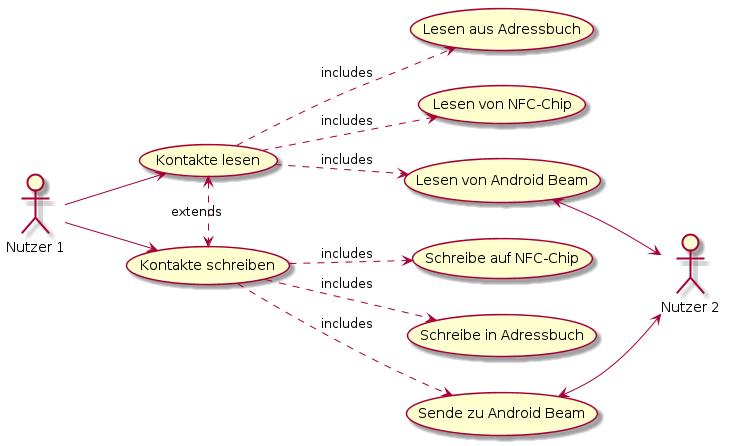
\includegraphics[width=\textwidth]{general_usecase.png}
\caption{Usecasediagramm}
\end{figure}

\section{Activity Diagramm}

Zu Beginn der Implementierung ist es wichtig, sich ausgehend vom Usecase Diagramm Klarheit über den logischen Aufbau der App zu machen, hier ist ein Aktivitätsdiagramm bestens geeignet. Hier werden auf übersichtliche Weise alle möglichen Bedienpfade der App aufgezeigt. Auch die innere Struktur der App ist entsprechend strukturiert.

 
\begin{figure}
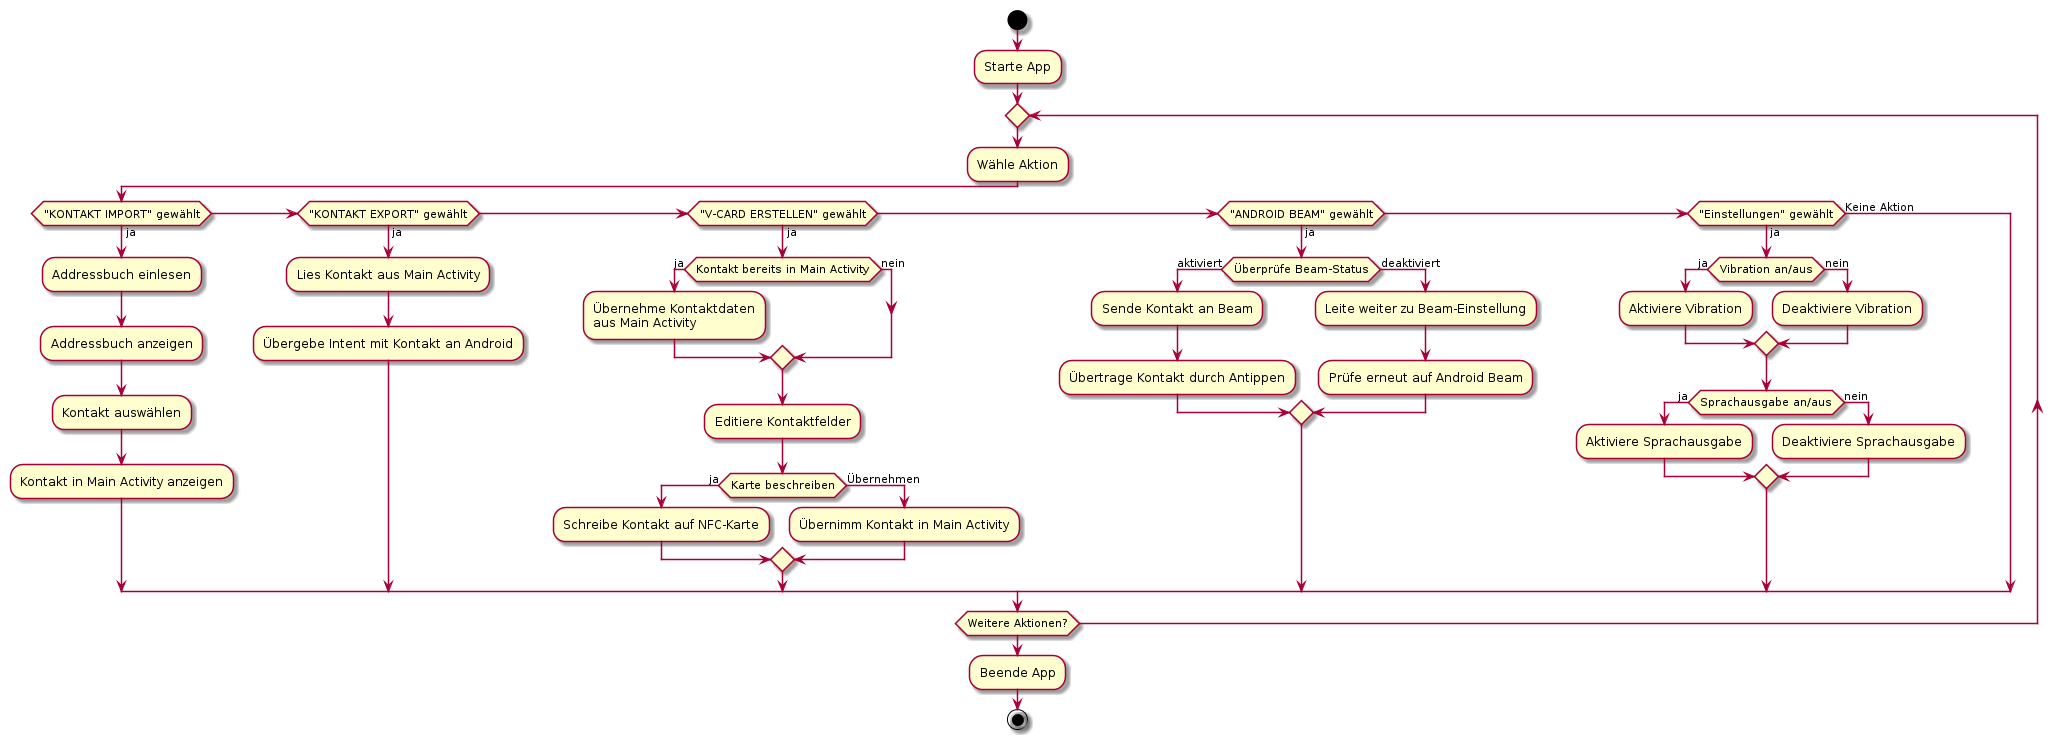
\includegraphics[width=\textwidth]{general_activity.png}
\caption{Aktivitätsdiagramm}
\end{figure}


\section{Klassendiagramm}

Nachdem die App auf die Bedienpfade abgestimmt wurde, ist es gute Praxis, die Funktionen logisch in verschiedene Klassen zu teilen. Anfangs wurde der Großteil in der Main Activity implementiert. Im Rahmen mehrerer Refactorings wurden immer mehr Funktionen in Klassen ausgelagert und diese in der Main Activity referenziert. Das zum Ende entstandene Klassendiagramm versucht die Abhängigkeit der Klassen untereinander aufzuzeigen.

 
\begin{figure}
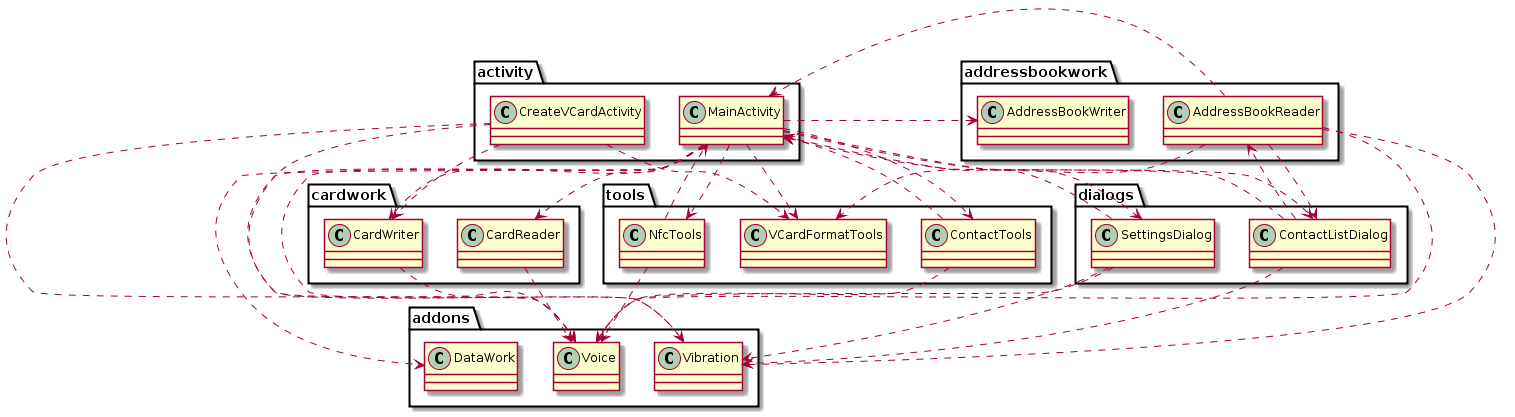
\includegraphics[width=\textwidth]{general_class.png}
\caption{Klassendiagramm}
\end{figure}

\chapter{Implementierung}
\section{Vorgehensweise}
\subsection{Extreme Programming}

Das Team arbeitete mit den agilen Methoden des „\+Extreme Programming“ (XP). Die Entscheidung zur Anwendung dieser Methode ist hauptsächlich durch den Projekttypen und die zu Projektbeginn zur Verfügung stehenden Informationen bedingt. \\
Da es sich um ein prototypisches Programmierprojekt handelt, war der Aufwand zur Implementierung einiger Funktionalitäten schwer abzuschätzen. Weiterhin war unser \char`\"{}\+Kunde\char`\"{}, Professor Schemmert, sehr gut verfügbar und auch in seinen Anforderungen flexibel.\\ Voraussetzung für die erfolgreiche Durchführung des XP waren der Einsatz einer verteilten Versionsverwaltung (siehe nächster Abschnitt), kontinuierliches Testen auf unterschiedlichen Geräten sowie eine teilautomatisch generierte Dokumentation.

Natürlich konnte nicht jede Technik genau nach diesem Modell angewandt werden, so waren beispielsweise „\+Stand Up Meetings“ nicht täglich sondern nur wöchentlich möglich.\\ 
Das Durchführen von „\+Unit Tests“ war ebenfalls zeitlich nicht realisierbar, zukünftig könnten diese aber durch den Einsatz von \char`\"{}\+\ac{Continuous Integration}\char`\"{} abgedeckt werden. \\
Jedoch hat die X\+P-\/\+Technik des Pair-\/\+Programming immer wieder geholfen, Fehler, Lösungen und Code-\/\+Optimierungen schnell zu finden und zu realisieren. \\
Auch der gegenseitige bedingte Wissenszuwachs, der in einem Hochschulprojekt mit im Vordergrund stehen sollte, war dadurch sehr groß.

\subsection{programmiertechnisches Vorgehen}

Das Team ist programmiertechnisch folgendermaßen vorgegangen\+: Es wurde zunächst überlegt welche Klassen und Methoden implementiert werden müssen, nachdem diese realisiert wurden und im späteren Verlauf Abhängigkeiten entstanden, wurden diese agil hinzugefügt. \\
Sollte eine Klasse oder Methode zu groß geworden sein, wurden diese durch \ac{Refactoring} in dafür sinnvolle kleinere Klassen und Methoden ausgelagert. Wenn neue Elemente implementiert wurden, wurde danach oder dabei immer direkt getestet, somit konnten wir große Fehlprogrammierungen effektiv vermeiden.

Am Ende des Projekts wurde noch ein großes Refactoring durchgeführt um dem Code eine gute Leserlichkeit zu verleihen. Dabei wurden unter anderem Klassen und Methoden ausgelagert um die Architektur zu verbessern und intuitiver zu gestalten. \\
Des Weiteren wurden Tests durchgeführt um letzte Logikfehler zu beseitigen und die Speichereffizienz so wie die Performance zu steigern. Dabei bedienten wir uns unter anderem der Tools „\+Inspect Code“ und dem Ressourcenmonitor, welche in Android Studio integriert sind.

\section{Technische Besonderheiten}

Im Verlauf der Entwicklung gab es einige technische Besonderheiten zu beachten. Einen guten Überblick dazu bietet ein Blick in die {\bfseries Android\+Manifest.\+xml} \begin{DoxyVerb}<?xml version="1.0" encoding="utf-8"?>
<manifest xmlns:android="http://schemas.android.com/apk/res/android"
    package="com.ag.mk.nfccardreadwrite">
\end{DoxyVerb}


Hier werden alle benötigten Berechtigungen der App aufgelistet. Einige Berechtigungen haben sich erst im Verlauf der Entwicklung ergeben, beispielsweise C\+A\+L\+L\+\_\+\+P\+H\+O\+NE und V\+I\+B\+R\+A\+TE. \begin{DoxyVerb}    <uses-permission android:name="android.permission.NFC" />
    <uses-permission android:name="android.permission.READ_CONTACTS" />
    <uses-permission android:name="android.permission.WRITE_CONTACTS" />
    <uses-permission android:name="android.permission.VIBRATE" />
    <uses-permission android:name="android.permission.CALL_PHONE" />
\end{DoxyVerb}


Hier erhält die App Zugriff auf den N\+F\+C-\/\+Chip. \begin{DoxyVerb}    <uses-feature
        android:name="android.hardware.nfc"
        android:required="false" />

    <application
        android:allowBackup="true"
        android:icon="@mipmap/tagger_logo"
        android:label="@string/app_name"
        android:supportsRtl="true"
        android:theme="@style/AppTheme" >
        <activity android:name=".activity.MainActivity" >
            <intent-filter>
                <action android:name="android.intent.action.MAIN" />

                <category android:name="android.intent.category.LAUNCHER" />
            </intent-filter>
            <intent-filter>
                <action android:name="android.nfc.action.NDEF_DISCOVERED" />

                <category android:name="android.intent.category.DEFAULT" />
\end{DoxyVerb}


Zum Schreiben von N\+D\+E\+F-\/\+Daten müssen die Daten auf dem Chip mit einem speziellen M\+I\+M\+E-\/\+Typ gespeichert werden. So können Kontaktdaten mit dem Standard-\/v\+Card M\+I\+M\+E-\/\+Typ geschrieben werden und das Android System verwaltet automatisch die damit registrierten Anwendungen, so würde sich in diesem Fall jede mit v\+Card registrierte App öffnen lassen, z.\+B. die Android Kontakte-\/\+App.

Wir haben uns bewusst gegen einen generischen M\+I\+M\+E-\/\+Typ entschieden und stattdessen unseren eigenen gebaut:  application/vnd.\+com.\+ag.\+mk.\+nfccardreadwrite.\+beam. Ein praktischer Nebeneffekt ist die auf einigen Geräten existierende Verknüpfung unbekannter M\+I\+M\+E-\/\+Typen mit dem Google Play\+Store. Hierbei ist es möglich, die App nur durch Auflegen auf eine N\+F\+C-\/\+Karte aus dem Play\+Store herunterzuladen, da nur diese den von uns defninierten M\+I\+M\+E-\/\+Typ unterstützt. \begin{DoxyVerb}                <data android:mimeType="application/vnd.com.ag.mk.nfccardreadwrite.beam" />
            </intent-filter>
            <intent-filter>
                <action android:name="android.nfc.action.TECH_DISCOVERED" />
                <action android:name="android.nfc.action.TAG_DISCOVERED" />

                <category android:name="android.intent.category.DEFAULT" />
            </intent-filter>

            <meta-data
                android:name="android.nfc.action.TECH_DISCOVERED"
                android:resource="@xml/tech" />
        </activity>
        <activity android:name=".activity.CreateVCardActivity" >
            <intent-filter>
                <action android:name="android.intent.action.SEND" />

                <category android:name="android.intent.category.DEFAULT" />
            </intent-filter>
\end{DoxyVerb}


Eine weitere Besonderheit ist das systemweite Eintragen der App als Empfänger für geteilte Kontakte. Dazu wird die App auf den zu empfangenden M\+I\+M\+E-\/\+Typ, hier für das Standard v\+Card-\/\+Format, registriert und kann nun den v\+Card-\/senden-\/\+Intent des Systems empfangen.

\begin{DoxyVerb}            <intent-filter>
                <action android:name="android.intent.action.SEND" />

                <category android:name="android.intent.category.DEFAULT" />

                <data android:mimeType="text/x-vcard" />
            </intent-filter>
        </activity>

        <meta-data
            android:name="com.google.android.gms.version"
            android:value="@integer/google_play_services_version" />

    </application>

</manifest>
\end{DoxyVerb}


Natürlich wäre es ohne weiteres möglich gewesen, unsere App auf den generischen v\+Card-\/\+M\+I\+M\+E-\/\+Typ zu registrieren, intern handelt es sich um die gleiche Datenstruktur. Allerdings haben wir uns an dieser Stelle für den \char`\"{}exklusiveren\char`\"{} Weg entschieden.

\section{Dokumentation}

Für die Dokumentation unserer Arbeit haben wir verschiedene Teilautomatische Open Source Lösungen verwendet. Zum Erstellen der Java Dokumentation haben wir Doxygen genutzt. Zum Erstellen der UML Diagramme plantuml, welches die Möglichkeit bietet, UML Diagramme mittels einfacher Textbeschreibung automatisiert zu erstellen. Beide Tools bieten unter anderem La\+TeX Dokumente als Ausgabeformat, welche wir als Basis für unsere Dokumentation verwendeten.

\section{Problembetrachtung}

\subsection*{Doppelter Intent}

Der Fehler, welcher das größte Fehlverhalten verursachte und leider auch nicht durch das Analysieren von Exceptions zu beseitigen war, weil er zum Teil logischer Natur entsprang, war jener einer ungenutzten implementierten Technologie im Intent-\/\+Filter „\+Iso\+Dep.\+class.\+get\+Name()“. \\
Er wies folgendes Verhalten auf\+: Wann immer ein N\+FC Medium an das Gerät gehalten, bzw. ein Beam Vorgang gestartet wurde, startete die App automatisch neu. \\
Erst durch das Entfernen der Funktion aus dem Intent-\/\+Filter, konnte dieser Fehler behoben werden.

\subsection*{Zugriff auf das Secure Element}

Zur Kommunikation mit Bezahlterminals und Zugangssystemen verfügen Android Smartphones über ein Secure Element innerhalb des N\+F\+C-\/\+Chips. In diesem Secure Element sind I\+Ds und Schlüssel einiger sicherheitskritischer Anwendungen gespeichert, weshalb der direkte Zugriff darauf (via A\+PI o.\+ä.) nicht möglich ist. \\
Es kann nur die Route zum und vom Secure Element angesprochen werden, d.\+h. die Daten werden z.\+B. von der App bereitgestellt und das Secure Element stellt die Sicherheitsfunktion bereit.

\subsection*{Kartenemulation}

Zur Emulation von Karten kann auch das Secure Element des Gerätes verwendet werden, hierbei ist jedoch zwischen den unterschiedlichen N\+F\+C-\/\+Chips zu unterscheiden, da diese nicht jeden Kartentyp emulieren können.\\
\+Zur Unterscheidung der N\+F\+C-\/\+Lesegeräte werden diese intern mit einer Typ-\/\+ID versehen und im Android-\/\+System entsprechend geroutet. Dieses Routing verhindert auch den weiteren Einsatz der Kartenemulation.\\ Das Hauptproblem hierbei ist das statische Routing der \ac{AID} auf spezielle Apps. 
Wenn es zu der A\+ID des Lesegerätes keine im System registrierte App gibt, dann kommt der initiale Handshake zwischen emulierter Karte und Lesegerät nicht zustande. 
Der Großteil der Hersteller verwendet eigene A\+I\+Ds und stellt diese meist nicht zur Verfügung, weiterhin werden diese A\+I\+Ds vom Android-\/\+System zwar registriert, aber sind nicht ohne erheblichen Aufwand (Änderung der Berechtigungsdatei mit root-\/\+Rechten...) auszulesen. \\
Folglich wäre es notwendig gewesen, die App auf mehrere A\+I\+Ds zu registrieren. Für die anfängliche Idee, die Hf\+T\+L-\/\+Zugangskarte zu emulieren, hätte selbst die Kenntnis der A\+ID nicht ausgereicht, da diese ein Secure Element beinhaltet und dieses von der \ac{HCE} nicht abgedeckt werden kann. \newpage
Ein weiteres Problem hinsichtlich der \ac{HCE} ist auch eine mangelnde Testumgebung, für realistische Tests wäre die Anschaffung eines N\+F\+C-\/\+Lesegerätes unumgänglich gewesen, da der in Android integrierte N\+F\+C-\/\+Lesemodus zu generisch ist und sich nicht auf spezielle A\+I\+Ds beschränkt. \\
Angenommen, die A\+ID steht zur Verfügung, dann kann eine Verbindung der emulierten Karte zum Lesegerät aufgebaut werden und der Datentransfer beginnt. 
Im Anschluss ist ein weiteres Problem zu erwarten, da das Lesegerät eine \ac{APDU} an die emulierte Karte schickt und von dieser eine valide APDU Response erwartet. \\
An dieser Stelle wäre erneut die Manipulation einer validen Verbindung nötig gewesen um die korrekte APDU Response auszulesen. In Anbetracht dieser technischen Einschränkungen haben wir uns gegen die Implementierung der Kartenemulation entschieden.

\section{Entwicklungsmodell}

Zur Umsetzung der Entwicklung wurde von Anfang an auf das verteilte Versionskontrollsystem git gesetzt. Ungetestete Funktionen wurden in Branches entwickelt und erst bei voller Funktion in den dadurch stabil gehaltenen Master integriert (\char`\"{}merged\char`\"{}). \\
Falls dieser Master doch einen fehlerhaften Zustand aufwies, so ließ sich dieser problemlos aufgrund der Commit-\/\+Beschreibungen auf einen funktionierenden Stand zurücksetzen. Um dies zu vermeiden erfolgte das Hochladen (\char`\"{}\+Commit \& Push\char`\"{}) in den Master erst nach vorherigem Testen der App. 

Als technische Umsetzung wurde der git-\/\+Hosting-\/\+Dienst Git\+Hub genutzt. Dort wurde eine Organisation erstellt die wiederum mehrere git-\/\+Verzeichnisse (\char`\"{}\+Repositories\char`\"{}) beinhaltet. \\
So wurden von Anfang an die App und die Dokumentation in unterschiedlichen Verzeichnissen versioniert. Weiterhin wurde die bei Git\+Hub integrierte Ticketverwaltung zur Projektsteuerung und Behebung von Fehlern eingesetzt.\\
Jedes Fehlerticket (Tag\+: \char`\"{}bug\char`\"{}) enthält eine Beschreibung des Fehlers und kann einem Bearbeiter zugewiesen werden. Zusätzlich wurden noch Verbesserungsvorschläge als Ticket erfasst (Tag\+: \char`\"{}enhancement\char`\"{}) und die Tickets verschiedenen Meilensteinen zugeordnet um eine bessere Terminierung zu erreichen. 

\chapter{Open Source und Lizenz}
\subsection*{Open Source}
Die Ersteller der App arbeiten alle mit Linux und unterstützen dessen Philosophie der freien Weitergabe von (Quell)offener Software. Da der Quelltext der App teil der Bewertungsgrundlage ist und wir die Plattform Github verwenden war Open Source von Anfang an Teil des Entwicklungskonzeptes. Das erleichtert nicht nur die kooperative Arbeit an der App sondern bietet auch anderen Menschen die Möglichkeit den von uns erstellten Quellcode zum Lernen zu nutzen und weiterzuentwickeln.

\subsection*{Lizenz}

Wir haben uns für die G\+P\+Lv2 (G\+NU General Public License) entschieden, welche die Nutzung, Bearbeitung und Weitergabe des von uns erstellen Quellcodes regelt. Die G\+P\+Lv2 existiert bereits seit 1991 und ist einer der am weitesten verbreiteten Softwarelizenzen für freie Software. Sie gestattet es dem Lizenznehmer die Software frei zu verwenden, bearbeiten und weiterzuverbreiten. Sie verpflichtet den Lizenznehmer dabei die Software nur mit dem selbigen Lizenzmodell weiterzugeben was eine kommerzielle Nutzung unseres Quellcodes weitestgehend ausschließt. 

\chapter{Arbeitsteilung}
\section*{Programmierung}

Oliver Friedrich\+: Beam Implementierung \\ 
Marko Klepatz\+: Main Activity, Helper Klassen, Refactoring, Bug-\/\+Fixing\\
Klaus Steinhauer\+: Android Kontakt Handeling\\ 

\section*{Dokumentation}

Oliver Friedrich\+: U\+ML, Planung, Implementierung\\
Marko Klepatz\+: Problemstellung, Quelltext Doku\\
Klaus Steinhauer\+: Ziel, Einleitung, Anforderungen, Lizenz, Fazit\\

\chapter{Fazit und Ausblick}

Im Laufe des Semesters konnten wir einen guten Einblick in die Android Programmierung gewinnen. Unsere Aufgabenstellung hat weite Teilbereiche der Android A\+PI abgedeckt und bietet damit eine gute Grundlage um tiefer in die Materie einzudringen. \\
Im Laufe des Semesters konnten wir Projektplanungs-\/ und Software-\/\+Engineering Kenntnisse aus den vergangenen Semestern praktisch anwenden und damit den planungsgemäßen Ablauf des Projektes sicherstellen.\\ 
Trotz unterschiedlicher Vorkenntnisse in der Android Programmierung konnten wir uns alle gut in die Programmierung einbringen und jeder einzelne einen Teil beitragen.

\section{Ausblick}

Die App ließe sich auf verschiedene Weisen erweitern. Das Unterstützen von Kontaktbildern wäre wünschenswert, sofern der Speicherplatz der Karte dies zulässt, und auch andere frei wählbare v\+Card Felder wären denkbar. \\ Sinvoll wäre zudem weitere Kartentypen zu unterstützen und die Kartensimulation in die Praxis umzusetzen. 

%--- End generated contents ---

% Index
\newpage
\phantomsection

\chapter{Anhang}
\section{Abkürzungsverzeichnis}
%Abkürzungen
\begin{acronym}
	\acro{HCE}{Host based card emulation: Emulation einer NFC-Karte durch das Gerät}
	\acro{APDU}{Application Protocol Data Unit: Anwendungseinheit innerhalb der NFC-Kommunikation, standardisiert nach ISO 7816}
	\acro{AID}{Application ID: eindeutige ID des NFC-Readers}
	\acro{NFC}{Near Field Communication: auf RFID basierender Übertragungsstandard}
	\acro{RFID}{radio-frequency identification: Technologie zur kontaktlosen Datenübertragung mittels elektromagnetischer Wellen}
	\acro{NDEF}{NFC Data Exchange Format, Standard-Datenaustauschformat zwischen NFC-Chips}
	\acro{Refactoring}{Begriff aus dem Software Engineering, Restrukturierung des Quellcodes zur besseren Lesbarkeit}
	\acro{Continuous Integration}{kontinuierliches Erstellen (Kompilieren) der Anwendung zur Steigerung der Softwarequalität}
\end{acronym}

\newpage
\begin{figure}
	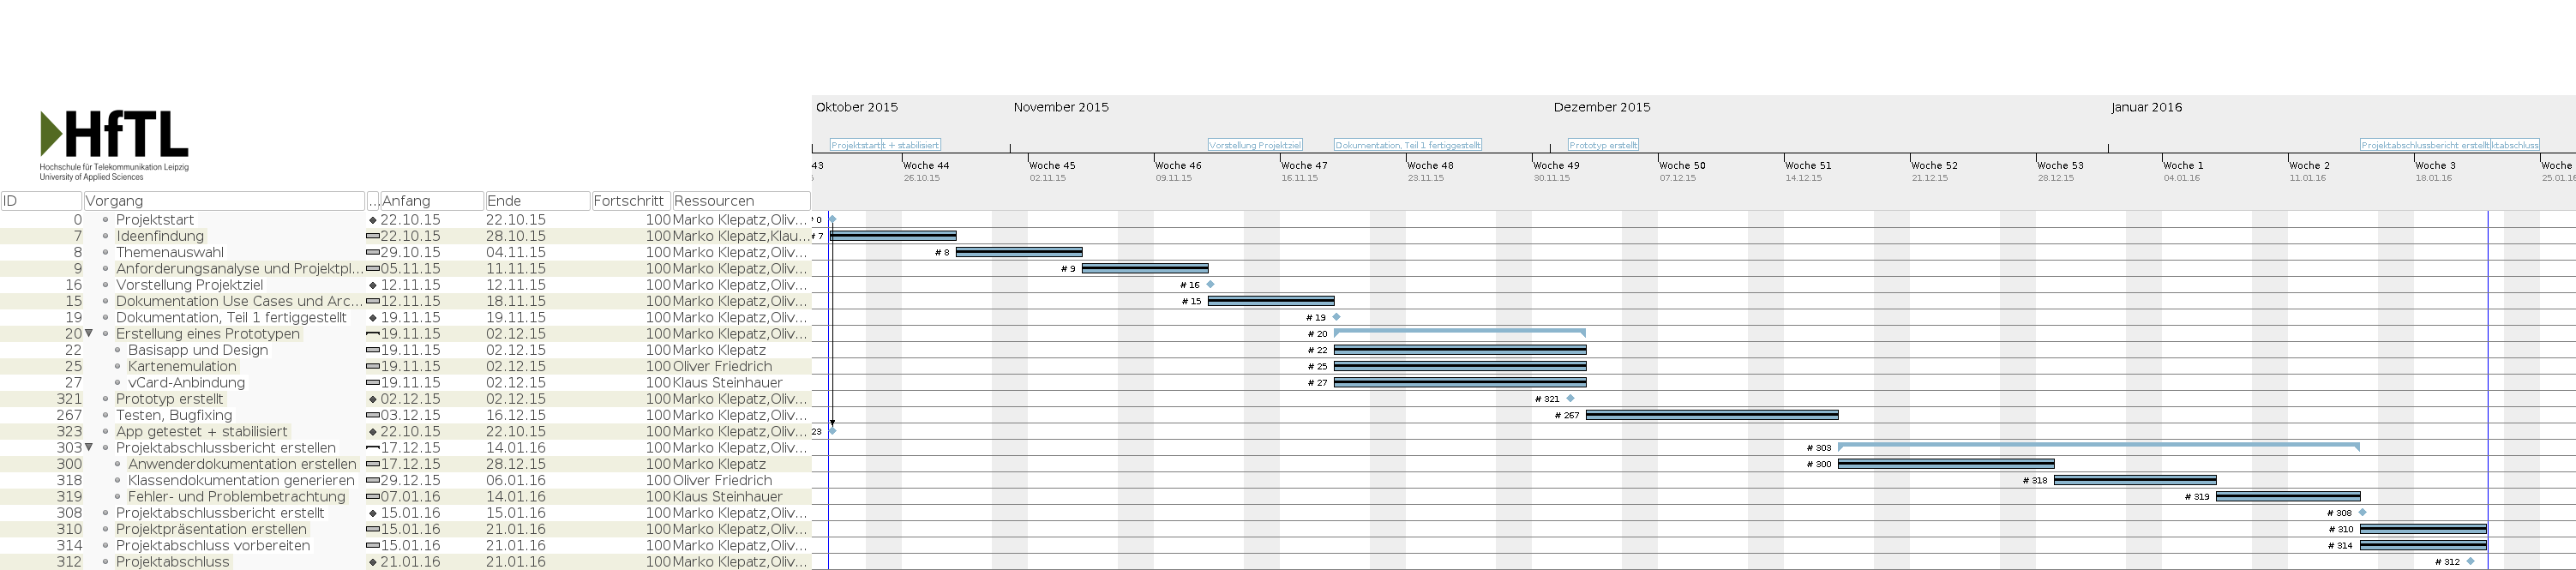
\includegraphics[width=\textheight, angle=90]{./project-mgmt/pplan.png}
	\caption{Projektplanung}
\end{figure}
\section{Quellenverzeichnis}
\nocite{*}
\printbibliography[heading=subbibliography,title={""}]
\newpage



\section{Programmcode Dokumentation}
\addtocontents{toc}{\protect\setcounter{tocdepth}{1}}
\newcommand*{\CommonPath}{./doxygen/latex}% 
\subsection*{Klassen-\/\+Dokumentation}
\input{\CommonPath/classaddressbookwork_1_1_address_book_reader}
\input{\CommonPath/classaddressbookwork_1_1_address_book_writer}
\input{\CommonPath/classtools_1_1_beam_tools}
\input{\CommonPath/classcardwork_1_1_card_reader}
\input{\CommonPath/classcardwork_1_1_card_writer}
\input{\CommonPath/classdialogs_1_1_contact_list_dialog}
\input{\CommonPath/classtools_1_1_contact_tools}
\input{\CommonPath/classactivity_1_1_create_v_card_activity}
\input{\CommonPath/classtools_1_1_data_work}
\input{\CommonPath/classactivity_1_1_main_activity}
\input{\CommonPath/classtools_1_1_nfc_tools}
\input{\CommonPath/classdialogs_1_1_settings_dialog}
\input{\CommonPath/classtools_1_1_v_card_format_tools}
\input{\CommonPath/classaddons_1_1_vibration}
\input{\CommonPath/classaddons_1_1_voice}
%--- End generated contents ---


\end{document}